\documentclass[12pt]{article}

\usepackage{xspace}
\usepackage{lineno}
\usepackage{setspace}
\usepackage{graphicx}
\usepackage{subfigure}
\usepackage{float}
\usepackage{color}
\usepackage{caption}
\usepackage[margin=1in]{geometry}
\usepackage{epstopdf}
\usepackage{natbib}
\usepackage{amsmath}
\usepackage{longtable}
\usepackage{booktabs}

\begin{document}
\doublespacing
\linenumbers


\newcommand{\Lik}{\ensuremath{\text{\emph{L}}}\xspace}
\newcommand{\selacDMS}{\emph{SelAC}+DMS\xspace}
\newcommand{\phydms}{\emph{phydms}\xspace}
\newcommand{\selac}{\emph{SelAC}\xspace}
\newcommand{\ecoli}{\textit{E. coli}\xspace}
\newcommand{\gy}{\emph{GY94}\xspace}
\newcommand{\PC}{physicochemical\xspace}  

\noindent RH: LANDERER ET AL.--- Estimating genetic load
% put in your own RH (running head)
% for POVs the RH is always POINT OF VIEW
\bigskip
\medskip
\begin{center}

% Insert your title:
\noindent{\Large \bf Experimentally informed phylogenetic models are biased towards laboratory conditions and can be improved upon by mechanistic models of stabilizing selection.}
\bigskip


\noindent{C\textsc{EDRIC} ~{L\textsc{ANDERER}}$^{1,2,*}$,
B\textsc{RIAN} C.~ {O\textsc{MEARA}}$^{1,2}$,
\textsc{AND}
M\textsc{ICHAEL} A.~{G\textsc{ILCHRIST}}$^{1,2}$}

\end{center}

\vfill

{\small
\noindent$^{1}$Department of Ecology \& Evolutionary Biology, University of Tennessee, Knoxville, TN 37996-1610\\
\noindent$^{2}$National Institute for Mathematical and Biological Synthesis, Knoxville, TN 37996-3410\\
\noindent$^{*}$Corresponding author. E-mail:~cedric.landerer@gmail.com
}

\vfill
\centerline{Version dated: \today}
\vfill
\newpage


\section{Introduction}
Phylogenetic inference is of ever increasing importance across biology \citep{omeara2006,YangAndBourne2009,Ruprecht2017,SchwartzAndSchaffer2017}. 
Most common models used for phylogenetic inference are incorporated into powerful software packages such as RAxML \citep{raxml}, RevBayes \citep{revbayes}, or IQTree \citep{nguyen2015}
While commonly used models are fast and easy to use, they lack biological realism.

Phylogenetic models focused on the nucleotide composition such as GTR, or UNREST \citep{Tavare1986,Yang1994} are limited to mutation effects and are agnostic to any higher level selection on codons or amino acids.
Amino acid models like JTT \citep{jones1992}, BLOSSUM \citep{blossum}, or WAG \citep{whelan2001} attempt to describe the effects of natural selection, however, these do not properly account for mutations between nucleotides and are purely phenomenological.
In an attempt to remedy the shortcomings of nucleotide and amino acid models, codon models combine mutation between nucleotides and selection on the amino acids for which they code.
Most popular, the codon model by \citet{GoldmanAndYang1994} (\gy) and its derivatives. 
However, \gy is commonly misinterpreted and only provides a restricted selection scenario that is best described as frequency dependent selection \citep{beaulieu2019}.

These types of models, weather they describe substitutions between nucleotides, codons, or amino acids, have in common that they describe the same equilibrium frequencies at each site without further modifications.
Biologists, however, have long recognized that equilibrium frequencies and thus the substitution matrix responsible, can vary substantially between sites \citep{felsenstein1981, gojobori1983}.
Individual sites along the sequence e.g. show differences in evolutionary rates, and wide range of preferences for specific amino acids \citep{HalpernAndBruno1998, ashenberg2013, echave2016}.
\citet{HalpernAndBruno1998} provided a general solution were each site can have a distinct substitution matrix.
As a result, the model introduced by \citet{HalpernAndBruno1998} had up to $19\times n$ parameters, where $n$ is the number of amino acid sites.
This large number of parameters that have to be estimated from the phylogenetic data makes the application of this model often unfeasible.

To overcome the issue of estimating an unfeasible amount of parameters from phylogenetic data, it was proposed to use additional data from deep mutation scanning experiments (DMS).
DMS allows for the estimation of site specific selection on amino acids for a large amount of mutations in a single experiment.
Using such external site specific selection estimates allows for the fitting of complex site specific models to smaller phylogenetic data sets, and it improves model fit \citep{bloom2014, bloom2017, hilton2017}.

However, such DMS estimates of selection are not always available.
The power of DMS stems from the ability to manipulate a large number of individuals in the laboratory and estimate genotype fitness based frequency changes over many generations.
This, however, limits the application of DMS selection estimates for phylogenetic inference greatly; to organisms with short generation times and that can be manipulated under laboratory conditions.
Laboratory conditions can greatly differ from the condition an organism experiences in the wild, therefore, it is questionable how well selection estimates inferred under such conditions reflect selection in the wild and are applicable for phylogenetic inference.
Selection estimates depend on factors like the initial library of mutations which - if extensive - leads to a heterogeneous population of competing individuals unlikely to be observed in the wild.
The selection applied in the laboratory is also likely to differ from the wild.
In addition, \citet{hilton2017} showed variation between DMS experiments can lead to significant differences in model inference.

Alternatively, better models could be be developed instead of using questionable external data for phylogenetic inference.
Lartillot and colleagues mitigate the high numbers of parameters by using a site categorization approach \citep{LartillotAndPhilippe2004,le2008}.
In this work we utilize \selac \citep{beaulieu2019} which uses a site categorization approach similar to the work by Lartillot and colleagues.
\selac utilizes a simplistic nested model and is rooted in population genetics.
The distance of amino acids in \PC space is used by \selac to describe the decline in fitness of an amino acids relative to an, for a site, optimal amino acid.
Therefore, \selac is limited to $20$ site categories, one for each possible optimal amino acid, but with a clear biological interpretation of each site category.

We assess the reliability of selection on amino acids inferred by DMS to inform phylogenetic studies.
We utilize a DMS experiment by \citet{stiffler2016} for the $\beta$-lactamase TEM.
TEM is an enzyme found in gram-negative bacteria like \textit{Escherichia coli} and catalyzes antibiotics with a $\beta$-lactam ring, providing antibiotic resistance \citep{Neu1969}.
The selection pressure imposed during the DMS experiment was limited to ampicillin and focused solely on the variant TEM-1 \citep{stiffler2016}.
However, TEM variants can also confer resistance to a wide range of other antibiotics \citep{sougakoff1988,sougakoff1989,goussard1991,mabilat1992,chanal1992,brun1994}.

Our results that site specific selection inferred by DMS improve model fit are consistent with previous work, but supplementing phylogenetic inference with unnatural data causes poor model adequacy. 
We use \phydms \citep{hilton2017} to fit 49 TEM sequences from \citet{bloom2017} using DMS inferred site specific selection on amino acids.
We compare the model fit of \phydms to \selac and find that model selection prefers \selac over \phydms.
Further, we find evidence that the DMS inference of selection on amino acids is inconsistent with selection on the wild at many sites, leading to poor model adequacy.
We do not observe the amino acid with the highest fitness estimated by DMS for $\sim 50 \%$ of sites.
We also find that the DMS estimates imply a very large genetic load of the observed TEM sequences.
In contrast, \selac shows higher model adequacy and a more realistic genetic load.

Together, our results show that  models can be more informative and applicable than unnatural supplementary data for phylogenetic inference.
\selac, in contrast, provides biological meaningful information such as site specific optimal amino acids and fitness landscape.
In addition, \selac does not rely on supplementary data and can be expanded to test other hypothesis.

\section{Results}
\subsection{\selac Outperforms Experimentally Informed Models}for 

Phylogenetic models of site specific selection on amino acids drastically improve model fit over classical nucleotide and codon models.
We compared \selac and \phydms to 131 nucleotide and 97 codon models and their variations (see Table \ref{tab:AIC_full} for all models).
\selac showed the best model fit and provided an improvement of 582 AIC units over the empirically informed model fit by \phydms despite the 272 more model parameters estimated from the phylogenetic data (Table \ref{tab:AIC_selac}). 
\phydms, parameterized by site specific selection estimates from citet{stiffler2016}, was performed second best and provided an improvement of 337 AIC units for the best non-site specific model, the symmetric model by \citet{zharkikh1994}. 

\begin{table}
  \centering
  \caption{Model selection, shown are the three models of stabilizing site specific amino acid selection (\selac, \phydms) and the best performing codon and nucleotide model \citep{GoldmanAndYang1994, zharkikh1994}. 
  Reported are the log-likelihood $\log(\Lik)$, the number of parameters estimated $n$, AIC, and $\Delta$AIC values.
  See Table \ref{tab:AIC_full} for results from all models we tested.}  
  \begin{tabular}{lrrrrrr}
    \hline
    Model							& $\log(\Lik)$ & n & AIC & $\Delta$AIC \\ \hline 
    \selac							& -1498 & 374 & 3744 &  0 \\
    \phydms 						& -2061 & 102 & 4326 & 582 \\
    \emph{SYM}+R2 				& -2230 & 102 & 4663 & 919 \\
    \emph{GY94}+F1X4+R2 		& -2243 & 102 & 4690 & 946 \\ \hline
  \end{tabular}
  \label{tab:AIC_selac}
\end{table}


The best performing codon model without site specific selection is \gy \citep{GoldmanAndYang1994}. 
However, \gy was outperformed by various nucleotide models like \emph{SYM}+R2.
Like \selac, \gy utilizes differences in \PC space between amino acids, but unlike \selac which is a model of stabilizing selection, \gy is best interpreted as frequency dependent selection \citep{beaulieu2019}.

We observe differences in the topology between model fits.
The \selac model is currently too slow to estimate the topology, therefore the topology was estimated using the codon model of \citet{KosiolEtAl07}.
\phydms uses the topology estimated with the codon model of \citet{KosiolEtAl07} as starting point for its topology search.
\phydms diverges from the initial topology suggesting we are conservative in our estimate of $\Delta AIC$ between \selac and \phydms.
However, at this point, it is therefore unclear if  we can attribute the difference in topology solely to the experimentally inferred selection or if other factors contribute.

IF WE UTILIZE THE \phydms INFERRED TOPOLOGY WITH \selac WE FIND THAT ....

Figure \ref{fig:phylo} shows that the estimated phylogenetic trees shift from long terminal branches (\selac) to longer internal branches (\phydms).
While the \selac model fit shows $84 \%$ of all evolution happening at the tips, this reduces $77 \%$ in the \phydms and \gy model fits.
All models produce polytomies but their location differs between models.
Surprisingly, the largest polytomies appear in the experimentally informed phylogeny of \phydms.


\singlespacing
\begin{figure}[H]
     \centering
	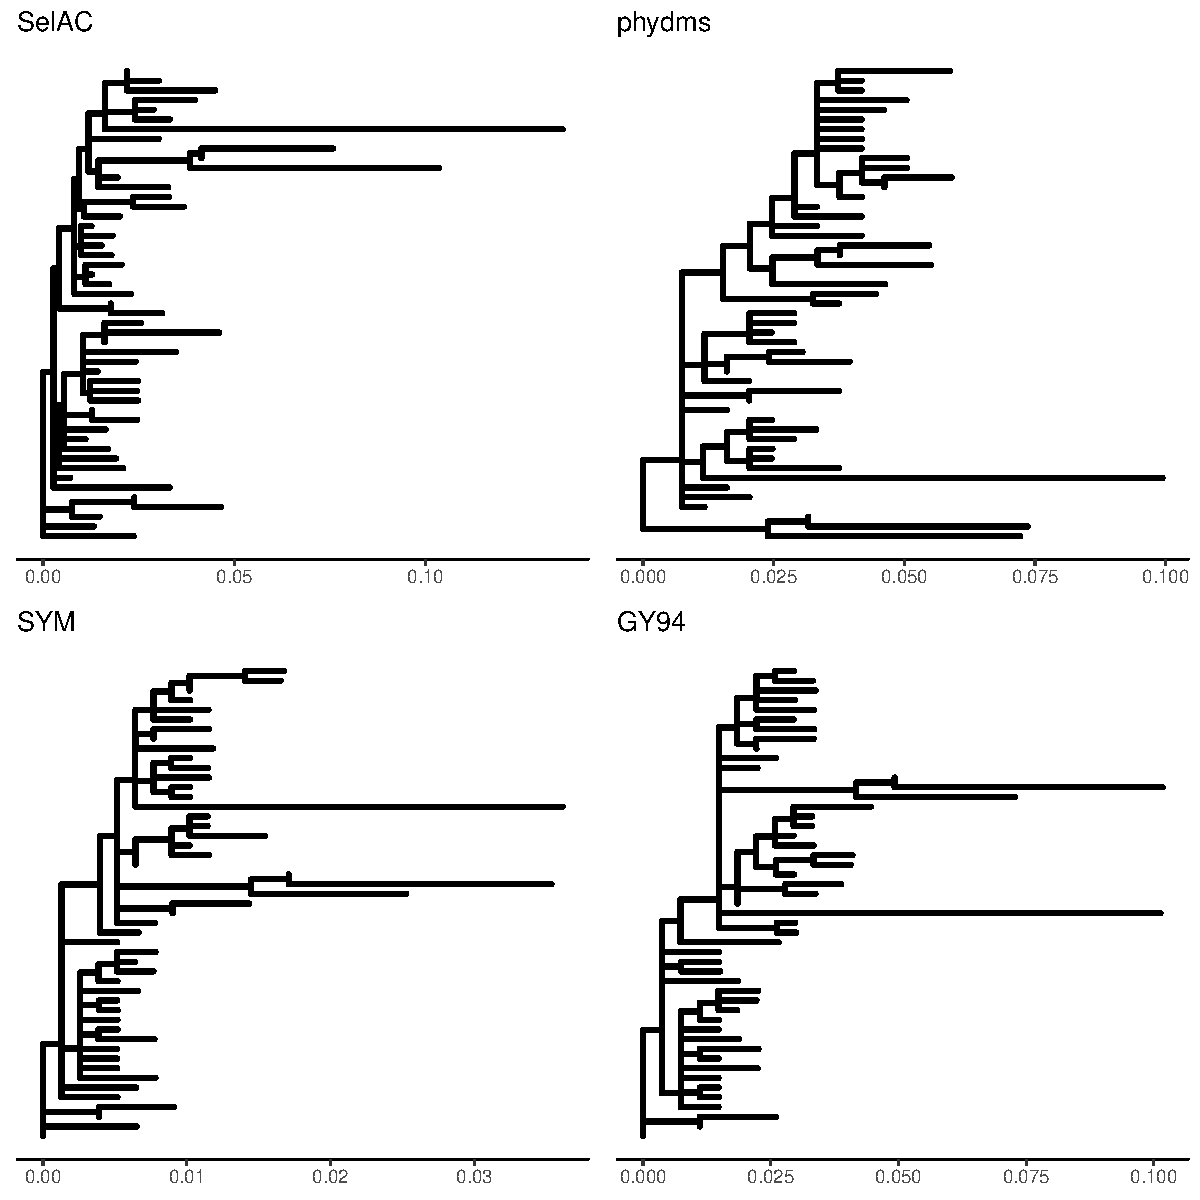
\includegraphics[width=\textwidth]{img/phy_TEM2016.pdf}
	\caption{REMOVE \selacDMS, ADD SYM INSTEAD Phylogenies resulting from \selac,\emph{SYM} , \phydms, and \gy. As \selac is currently to slow for the inference of topologies, the topology for the \selac phylogeny was inferred using the codon model of \citet{KosiolEtAl07}.}
	\label{fig:phylo}
\end{figure}
\doublespacing
\clearpage

\subsection{DMS Leads to Poor Model Adequacy And Predictions Inconsistent with Observed Genetic Variation in TEM}

We define model adequacy as similarity of selectively favored amino acids and observed consensus sequence.
The sequence of selectively favored amino acids experimentally estimated by DMS shows a low sequence similarity of only $52 \%$ with the observed consensus sequence. 
We find that the selectively favored amino acid estimated by DMS is not found in the wild in X \% of sites.
Additionally, the \PC properties appear to differ between the observed and the DMS estimated optimal amino acids.
Together this suggests that DMS selection estimates are not very informative about selection in the wild.

In contrast, the \selac model fit shows high model adequacy.
The \selac inferred sequence of selectively favored amino acids has $99 \%$ sequence similarity with the observed consensus sequence.
This may not be to surprising given that \selac only used the phylogenetic data and no experimental supplementary data.

\begin{table}
  \centering
  \caption{Genetic load at variant and invariant sites in the TEM alignment according to \selac and DMS}
  \begin{tabular}{lccc}
    \hline
			& 		& \multicolumn{2}{c}{Genetic Load}  \\ 
    Sites 		& \# Residues	& \multicolumn{1}{c}{\selac} & \multicolumn{1}{c}{DMS} \\ \hline 
    Variant	&	66	& $6.3\times10^{-7}$ & 0.010  \\
    Invariant		& 	197	& 0 & 0.007 \\
  \end{tabular}
  \label{tab:selection}
\end{table}

We further find that the genetic load is inconsistent with the observed genetic variation in TEM.
For example, \selac predicts a zero genetic load at invariant sites, while the genetic load predicted at these sites is not significantly different from the genetic load at the variant sites (Table \ref{tab:selection}).
This shows that the distribution of genetic load differs between DMS inferred site specific selection and \selac inferred site specific selection.
If we assume the site specific selection estimated by DMS, 111 sites show no genetic load.
In contrast, if we assume the site specific selection estimated by \selac, 207 sites show no genetic load.
The \selac estimates of selection are more in line with the observed sequences as only 66 sites show genetic variation.

In total, we find 100 sites for which estimates a genetic load of zero but the DMS estimates predict a non-zero genetic load.
All 100 cases show a significant difference in the likelihood between the \selac and the DMS inferred optimal amino acid.
In addition, these 100 sites show a significant higher genetic load than the remaining 163 sites of $0.0157$ and $0.003$, respectively ($p = 3\times10^{-13}$).

For 52 sites, both DMS and \selac estimate a non-zero genetic load.
in 26 cases, the same optimal amino acid is predicted, in the remaining 26 cases DMS predicts a significantly different optimal amino acid.
Again we find a significant difference in genetic load between the 26 for which the \selac and DMS predictions of the optimal amino acid agree and the 26 sites for which they differ of $0.004$ and $0.0158$, respectively ($p = 2\times10^{-5}$).

\subsection{DMS Implies Unrealistic Genetic Loads}

As indicated previously, the genetic load of the observed TEM sequences differs greatly under the \selac and experimentally estimated fitness landscape.
The site specific selection estimated by DMS for the observed TEM sequences represents an average site specific load of 0.065.
In contrast, the site specific genetic load estimated by \selac for the observed TEM sequences represents an average site specific genetic load of only $2.4\times 10^{-7}$.

\begin{figure}
    \centering
    \begin{subfigure}
        \centering
        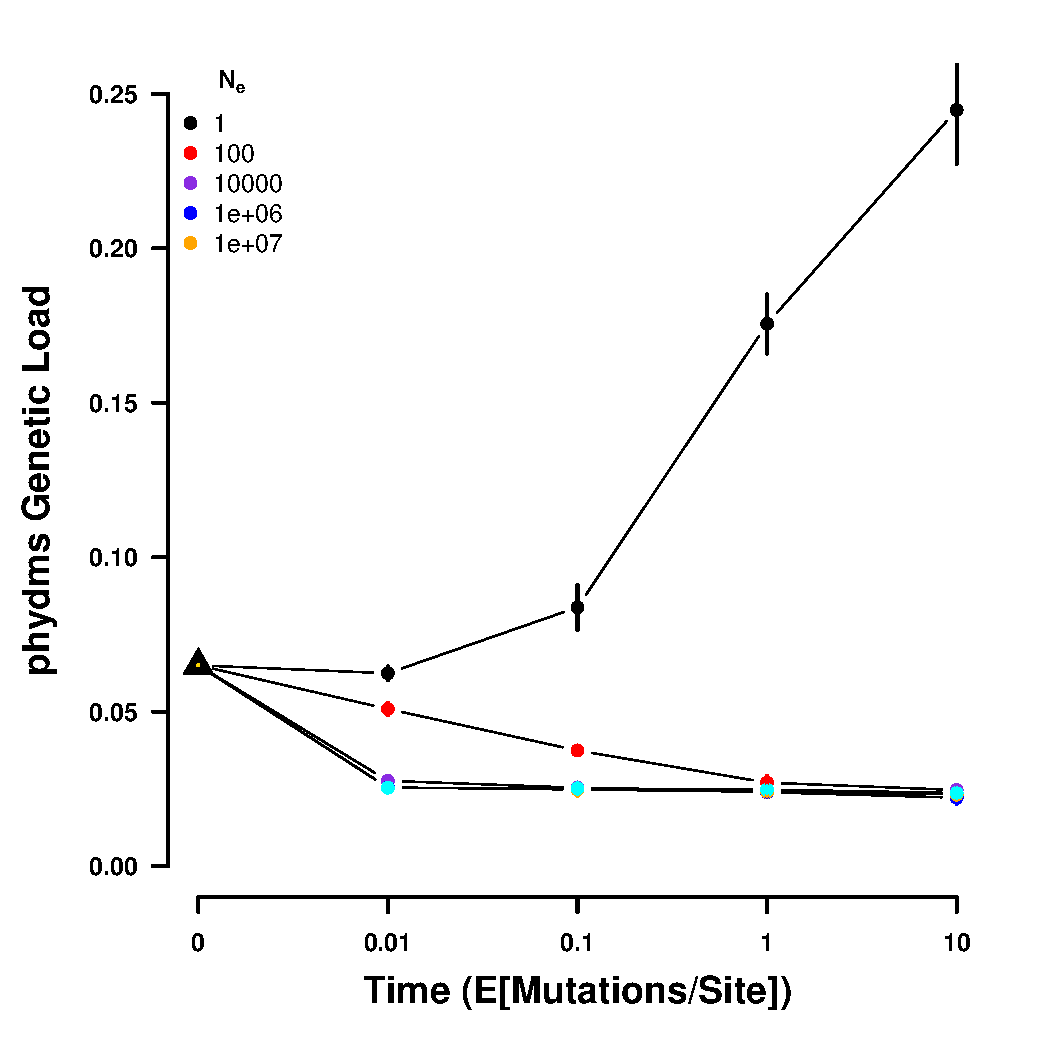
\includegraphics[width=.45\textwidth]{img/simulated_gl_time_DMS_ancest.pdf}
    \end{subfigure}
    \begin{subfigure}
        \centering
        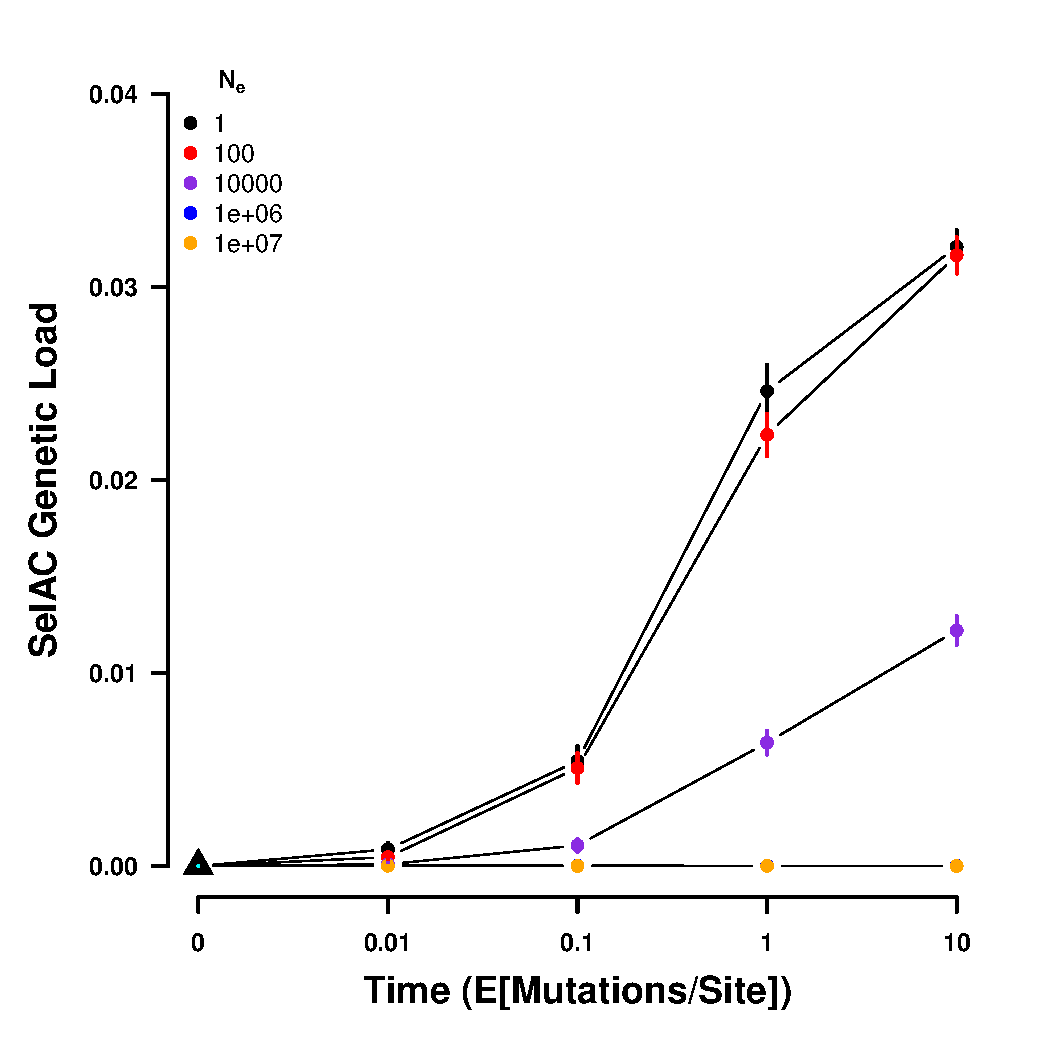
\includegraphics[width=.45\textwidth]{img/simulated_gl_time_SELAC_ancest.pdf}
    \end{subfigure}
    \caption{Sequences simulated from the ancestral state under the site specific selection on amino acids estimated using deep mutation scanning. 
    (left) and \selac (right) at various times for a range of $N_e$ values.
    Time is given in number of expected mutations per site, which equals the substitution rate of a neutral mutation.
    Points indicate sample means and vertical bars indicate standard deviations. Initial sequence is the inferred ancestral state of the TEM variants and indicated by a black triangle.}
    \label{fig:gl_sim}
\end{figure}


We simulated sequences forward in time from the ancestral state under the DMS and \selac inferred selection to establish a point of reference and further assess model adequacy (Figure \ref{fig:gl_sim}).
Simulations under the DMS inferred selection show that the genetic load of the observed sequences is larger than the genetic load of the simulated sequences.
The simulations yield an average site specific genetic load of 0.025.
Simulations under the \selac inferred selection as well show that the genetic load of the observed sequences is larger than the genetic load of the simulated sequences.
The simulations yield an average site specific genetic load of $1.3 \times 10^{-5}$

\section{Discussion}

We compared the performance of two codon level phylogenetic models with site specific selection, \phydms and \selac, as well as 230 more commonly used codon and nucleotide models in explaining TEM data.
We used 49 TEM sequences obtained from \citet{bloom2017}.
Using AIC as measure of model fit we find that both models of site specific selection, \phydms and \selac perform substantially better that the alternative models, including the classic model from \citet{GoldmanAndYang1994}.
Further, we find that \selac outperforms \phydms substantially ($\Delta AIC = 582$).

The improved performance of \phydms and \selac presumably results from their ability to more realistically describe the effects of natural selection on sequence evolution.
However, this realism comes at a cost. 
\phydms requires supplementary fitness estimates for each amino acid at every site, which necessitates experimental work.
\selac, on the other hand, uses a nested modeling approach, which avoids the necessity of amino acid specific fitness estimates, but greatly increases the computational cost of model fitting.

We further assessed the model adequacy of \phydms and \selac which we primarily define as the similarity of the sequence of optimal amino acids to the observed consensus sequence.
While the consensus sequence ignored the phylogenetic relationship between the sequences, it is a still good metric to assess the realism of the estimated optimal amino acids as it provides a summary of the amino acids observed in the wild.
However, we also assessed the genetic load of the observed sequences according to the DMS and \selac estimates fitness landscape.
Model adequacy is a measure that describes how well observed data can be reproduced by a model and is often ignored.
The model adequacy of \phydms is a direct function of the supplementary DMS measurements. 
As a result, we focused directly on these measurements.

Like model selection, model adequacy strongly favors \selac.
When model adequacy is assessed by sequence similarity the sequence of optimal amino acids and therefore the highest fitness estimated DMS has only 49 \% sequence similarity while the \selac estimated sequence shows a sequence similarity of 99 \% with the observed consensus sequence.
Given these results, it is tempting to assume that the consensus sequence will always fair best, however, this would assume independence between the observed sequences.
Furthermore, the high sequence similarity between the consensus sequence and the sequence of optimal amino acids is likely due to the high average sequence similarity in the TEM alignment of 98 \%.

Similarly, we find the genetic load of the DMS sequences is substantially higher when assuming the DMS estimated fitness landscape compared to the \selac estimated one with 0.065 and  $2.4\times 10^{-7}$, respectively.
However, if we assume that the DMS inference adequately reflects the evolution of TEM in the wild the observed sequences are either maladapted of were unable to reach a fitness peak.
This, however is unlikely as \ecoli has a large effective population size.
Estimates are on the order of $10^8$ to $10^9$ \citep{OchmanAndWilson1987,hartl1994}.
We would therefore expect that \ecoli can effectively explore the sequence space.
More specifically, assuming a mutation rate of $2.54\times 10^{-10}$ mutations per generation per nucleotide \citep{lee2012}, we would expect to find $2\times 10^{-7}$ mutations per generation in the 789 nucleotide long TEM sequence.
This results in between $\mu N_e = 10^1$ to $10^2$ mutations per generations throughout the population.
The average site specific selection against the observed TEM sequences is $s = 0.085$, we would therefore expect that mutations should fix on average within $(4/|s|)\times \ln(2 N_e) \sim 1200$ to 1300 generations \citep{CrowAndKimura1970}.
Given \ecoli's rapid doubling time of 15 hours in the wild \citep{gibson2018}, we would expect that an average mutation should sweep through the population in 1.5 years.

In contrast, estimates of selection obtained by \selac show the observed sequences at a fitness peak.
This is consistent with theoretical population genetics results.
It, therefore, appears that DMS reflects the biased laboratory selection on the TEM sequences with respect to only one antibiotic. 
This may be appropriate to model selection in a hospital environment but not when the interests lies in the evolution of TEM in the wild.
The evidence we derived from population genetics theory has us expecting the observed sequences at the selection-mutation-drift equilibrium.
This, however, is clearly not the case if we assume the DMS inferred selection.

Besides relatively poor performance in terms of model adequacy, DMS has additional shortcomings that limit its use in phylogenetic studies.
Like with any other experiments, results can greatly vary.
\citet{hilton2017} showed that a similar experiment to the one used here performed wore in explaining the observed data.
DMS experiments are also costly and limited to microorganisms that can be cultivated and manipulated under laboratory conditions.
These laboratory conditions can lead to the bias in selection estimates we observe in this study.

The artificial selection environment in the laboratory leads to a very heterogeneous population and very large selection coefficients $s$ unlikely to be observed in the wild.
The very large singular selection may be the easiest issue to overcome in DMS experiments as it may be possible to include a multitude of weaker selective forces.
However, this is often not the goal when performing DMS experiments as they were initially not intended for the use in phylogenetic studies but appropriated.
\selac on the other hand, better explains the evolution of TEM in the wild and does not require the supplementary selection data but provides such estimates.
This makes \selac also applicable to any set of aligned protein coding sequences.

However, \selac is  not without shortcomings itself, but its mechanistic nature provides direct avenues to overcome these via model expansion.
\selac assumes the same optimal amino acid at a site along the whole phylogeny.
Incorporation of a hidden markov model would not only allow for shifts in the optimal amino acid along the phylogeny but also relax the assumption of stabilizing selection.
In particular, a hidden markov approach would allow for frequency dependent selection like it is modeled by \gy which may be appropriate for TEM as it plays a role in chemical warfare between microorganisms.
However, our results and the high number of invariant sites in the alignment indicate that such frequency dependent selection may only applies to a small number of sites.

In order to map the amino acid sequence to protein fitness \selac uses the euclidean distance in \PC space between amino acids. 
A more realistic mapping could be employed by adding higher order terms or my utilizing an explicit molecular model.
\selac also currently ignores selection on synonymous codon usage and therefore treats synonymous mutations as neutral.

Other shortcomings of \selac with a less clear solution include the relaxation of the constrained that the site specific sensitivity of selection has to be positive.
Allowing for a negative sensitivity term would extend \selac to diversifying selection on amino acids.
The inclusion of a mixture model  where model parameters vary between site categories would allow to distinguish e.g. sites under stabilizing and diversifying selection.
Finally, \selac, like all other models considered here, assumes site independence, and thus ignores epistatic interaction between amino acids.

DMS experiments have been proposed to supplement information on selection on amino acids in phylogenetic studies.
This study shows that information on selection on amino acids does not have to be supplemented but can be extracted from alignments of protein coding sequences using a carefully constructed model of stabilizing selection rooted in first principles.
Further, we highlight the bias of laboratory estimates of selection and suggest to focus efforts in improving phylogenetic inferences on the development of more realistic models.
Better models can avoid many of the problems of supplementary data outlined in this study.
The ability to expand \selac as outlined above make it a valid starting point for such improvements and allow for explicit hypothesis testing.

\section{Materials and Methods}

\subsection{Phylogenetic Inference and Model selection}

TEM and SHV sequences were obtained from \citet{bloom2017} already aligned.
We separated the TEM and SHV sequences into individual alignments.
Experimentally fitness values for TEM were taken from \citet{stiffler2016}.
We followed \citep{bloom2017} to convert the experimental fitness values into site specific equilibrium frequencies for \phydms. 
\phydms (version 2.5.1) was fitted to the site specific selection from \citet{stiffler2016} using python (version 3.6).
\selac (version 1.6.1) was fitted to the TEM alignment using R (version 3.4.1) \citep{rcore} with and without experimental site specific selection.
We assumed the \PC properties estimated by \citet{grantham1974}.
We choose the constraint free general unrestricted model \citep{Yang1994} as mutation model for \selac.
All other models were fitted using IQTree \citep{nguyen2015}.
We report each model's $\log(\Lik)$, and AIC.
Models were selected based on the AIC values.

\subsection{Sequence Simulation}

Sequences were simulated by stochastic simulations using a Gillespie algorithm \citep{gillespie1976} that was model independent.
To calculate fixation probabilities during the simulation we followed \citet{SellaAndHirsh2005}.
The fitness values were estimated using \selac or taken from \citet{stiffler2016}.
We choose the fitness values resulting from the highest concentration (2500 $\mu g/mL$) treatment of ampicillin for our comparison.
We rescaled the experimental fitness such that the amino acid with the highest fitness at each site has a value of one.
Mutation rates for the simulations were taken from the \selac or \selacDMS fit, respectively.
The initial sequences were either a random sequence sampled with uniform codon probabilities or the ancestral sequence reconstructed using FastML \citep{fastml} (last accessed: 30.09.2018).
Each sequence was simulated 10 times and we report average genetic load and sequence similarity and the standard error.
The sequences were sampled at times 0.01, 0.1, 1, and 10 expected mutations per site.

%\subsection{Estimating site specific efficacy of selection $G$}

%\selac does not by default estimate site specific values for $G$ but assumes $G$ values follow a $\Gamma$-distribution \citep{Felsenstein2001}.
%Site specific values for $G$ were optimized by fixing all estimated parameters and performing a maximum likelihood search without the integration over $G$.
%In contrast to \selac that assumes $G$ to be purely positive, we allowed negative values for $G$ but constraint the search to values between $-300$ and $300$ to ensure numerical stability.

\subsection{Estimating site specific fitness values $w_i$}

Following \citet{beaulieu2019} $w_i$ is proportional to
\begin{equation}
w_i \propto \exp(-A_0\eta\psi)
\end{equation}
where $A_0$ describes the decline in fitness with each high energy phosphate bond wasted per unit time, and $\psi$ is the protein's production rate.
$\eta$ is the cost/benefit ratio of a protein (see \citep{beaulieu2019} for details). 
However, \selac only estimates a composition parameter $\psi' = A_0\psi N_e$ thus
\begin{equation}
\psi = \frac{\psi'}{A_0N_eq}
\end{equation}
\selac assumes that the effective population size $N_e = 5\times 10^6$ and that $A_0 = 4 \times 10{-7}$ \citep{gilchrist2007}.

\subsection{Model Adequacy}

Model adequacy was assessed by comparing the observed sequences and simulations under the site specific selection inferred by the deep mutation scanning experiment or \selac.
First, similarity between the sequence of selectively favored amino acids and the observed TEM sequences was assessed.
Sequence similarity was measured as the number of differences in the aligned amino acid sequences.
Second, the genetic load of the observed and the simulated sequences was calculated using either the site specific selection inferred by the deep mutation scanning experiment or \selac.
The average genetic load for site $i$ in the alignment was calculated as
\begin{equation}
L_i = \frac{w_{max,i} - \overline{w_i}}{w_{max,i}}
\end{equation}
where $w_{max,i}$ is the fitness of the selectively favored amino acids at position $i$, either estimated using the site specific selection inferred by DMS or \selac.
We, however, rescaled all fitness estimates such that $w_{max,i} = 1$
$\overline{w_i}$ represents the average fitness of the residues observed at position $i$.
The average sequence specific genetic load $L$ was calculated as the sum of the site specific genetic loads $L = \frac{1}{n}\sum_{i=1}^n L_i$ where $n$ is the number of amino acid sites.

\section{Acknowledgments}

This work was supported in part by NSF Award and DEB-1355033 (BCO, MAG, and RZ) with additional support from The University of Tennessee Knoxville. 
CL received support as a Graduate Student Fellow at the National Institute for Mathematical and Biological Synthesis, an Institute sponsored by the National Science Foundation through NSF Award DBI-1300426, with additional support from UTK. 
The authors would like to thank Russel Zaretzki, Jeremy Beaulieu and Alexander Cope for their helpful criticisms and suggestions for this work.



\bibliographystyle{natbib} \bibliography{ecoli}

\clearpage
%\beginsupplement
\section{Appendix: Supplementary Material}

\singlespacing
\begin{longtable}{clrrrrrr}
  \caption{Model selection of 230 models of nucleotide and codon evolution.}
  \label{tab:AIC_full}
  \\ 
  \toprule
  No. & Model & LnL & n & AIC & $\Delta$AIC & AICc & $\Delta$AICc \\   \hline \endfirsthead
  \caption*{Table \ref{tab:AIC_full} Continued}\\\toprule
  No. & Model & LnL & n & AIC & $\Delta$AIC & AICc & $\Delta$AICc \\   \hline \endhead
  \hline \endfoot
  \bottomrule
  \endlastfoot

	1 & \selacDMS+G4 & -1768 & 111 & 3758 & 14 & 3760 & 0 \\ 
	2 & \selac+G4 & -1498 & 374 & 3744 & 0 & 3766 & 6 \\ 
	3 & \phydms & -2060.85 & 102 & 4326 & 582 & 4328 & 568 \\ 
	4 & SYM+R2 & -2229.616 & 102 & 4663.232 & 919.232 & 4693.862 & 933.862 \\ 
	5 & TIMe+R2 & -2232.406 & 100 & 4664.811 & 920.811 & 4694.172 & 934.172 \\ 
	6 & TVMe+R2 & -2232.838 & 101 & 4667.677 & 923.677 & 4697.668 & 937.668 \\ 
	7 & TIM3e+R2 & -2234.332 & 100 & 4668.664 & 924.664 & 4698.024 & 938.024 \\ 
	8 & TIM2e+R2 & -2234.381 & 100 & 4668.763 & 924.763 & 4698.123 & 938.123 \\ 
	9 & K3P+R2 & -2235.777 & 99 & 4669.553 & 925.553 & 4698.291 & 938.291 \\ 
	10 & TNe+R2 & -2236.078 & 99 & 4670.155 & 926.155 & 4698.892 & 938.892 \\ 
	11 & SYM+R3 & -2229.616 & 104 & 4667.232 & 923.232 & 4699.162 & 939.162 \\ 
	12 & TIM+F+R2 & -2230.958 & 103 & 4667.915 & 923.915 & 4699.191 & 939.191 \\ 
	13 & TIMe+R3 & -2232.404 & 102 & 4668.808 & 924.808 & 4699.437 & 939.437 \\ 
	14 & GTR+F+R2 & -2228.537 & 105 & 4667.073 & 923.073 & 4699.665 & 939.665 \\ 
	15 & K3Pu+F+R2 & -2232.617 & 102 & 4669.234 & 925.234 & 4699.864 & 939.864 \\ 
	16 & TVM+F+R2 & -2230.105 & 104 & 4668.21 & 924.21 & 4700.14 & 940.14 \\ 
	17 & TVMe+R3 & -2232.838 & 103 & 4671.676 & 927.676 & 4702.952 & 942.952 \\ 
	18 & K2P+R2 & -2239.424 & 98 & 4674.847 & 930.847 & 4702.969 & 942.969 \\ 
	19 & TIM3e+R3 & -2234.332 & 102 & 4672.664 & 928.664 & 4703.293 & 943.293 \\ 
	20 & TIM2e+R3 & -2234.381 & 102 & 4672.762 & 928.762 & 4703.391 & 943.391 \\ 
	21 & TIM3+F+R2 & -2233.064 & 103 & 4672.127 & 928.127 & 4703.403 & 943.403 \\ 
	22 & TIM2+F+R2 & -2233.114 & 103 & 4672.227 & 928.227 & 4703.503 & 943.503 \\ 
	23 & K3P+R3 & -2235.777 & 101 & 4673.553 & 929.553 & 4703.545 & 943.545 \\ 
	24 & TN+F+R2 & -2234.624 & 102 & 4673.249 & 929.249 & 4703.878 & 943.878 \\ 
	25 & TPM3u+F+R2 & -2234.673 & 102 & 4673.347 & 929.347 & 4703.977 & 943.977 \\ 
	26 & TPM3+F+R2 & -2234.674 & 102 & 4673.348 & 929.348 & 4703.978 & 943.978 \\ 
	27 & TPM2u+F+R2 & -2234.681 & 102 & 4673.363 & 929.363 & 4703.993 & 943.993 \\ 
	28 & TPM2+F+R2 & -2234.683 & 102 & 4673.365 & 929.365 & 4703.995 & 943.995 \\ 
	29 & TNe+R3 & -2236.077 & 101 & 4674.155 & 930.155 & 4704.146 & 944.146 \\ 
	30 & TIM+F+R3 & -2230.958 & 105 & 4671.915 & 927.915 & 4704.507 & 944.507 \\ 
	31 & HKY+F+R2 & -2236.266 & 101 & 4674.531 & 930.531 & 4704.522 & 944.522 \\ 
	32 & GTR+F+R3 & -2228.536 & 107 & 4671.073 & 927.073 & 4705.011 & 945.011 \\ 
	33 & K3Pu+F+R3 & -2232.617 & 104 & 4673.234 & 929.234 & 4705.163 & 945.163 \\ 
	34 & TVM+F+R3 & -2230.105 & 106 & 4672.21 & 928.21 & 4705.471 & 945.471 \\ 
	35 & K2P+R3 & -2239.192 & 100 & 4678.384 & 934.384 & 4707.745 & 947.745 \\ 
	36 & TIM3+F+R3 & -2233.063 & 105 & 4676.127 & 932.127 & 4708.718 & 948.718 \\ 
	37 & TIM2+F+R3 & -2233.113 & 105 & 4676.227 & 932.227 & 4708.818 & 948.818 \\ 
	38 & TN+F+R3 & -2234.624 & 104 & 4677.249 & 933.249 & 4709.178 & 949.178 \\ 
	39 & TPM3u+F+R3 & -2234.673 & 104 & 4677.347 & 933.347 & 4709.277 & 949.277 \\ 
	40 & TPM3+F+R3 & -2234.674 & 104 & 4677.348 & 933.348 & 4709.277 & 949.277 \\ 
	41 & TPM2u+F+R3 & -2234.681 & 104 & 4677.363 & 933.363 & 4709.293 & 949.293 \\ 
	42 & TPM2+F+R3 & -2234.682 & 104 & 4677.364 & 933.364 & 4709.294 & 949.294 \\ 
	43 & HKY+F+R3 & -2236.074 & 103 & 4678.148 & 934.148 & 4709.424 & 949.424 \\ 
	44 & SYM+I+G4 & -2243.212 & 102 & 4690.424 & 946.424 & 4721.054 & 961.054 \\ 
	45 & TVMe+I+G4 & -2244.533 & 101 & 4691.066 & 947.066 & 4721.057 & 961.057 \\ 
	46 & TIMe+I+G4 & -2246.457 & 100 & 4692.914 & 948.914 & 4722.275 & 962.275 \\ 
	47 & K3P+I+G4 & -2248.166 & 99 & 4694.332 & 950.332 & 4723.069 & 963.069 \\ 
	48 & TVM+F+I+G4 & -2241.853 & 104 & 4691.707 & 947.707 & 4723.636 & 963.636 \\ 
	49 & TIM3e+I+G4 & -2247.379 & 100 & 4694.758 & 950.758 & 4724.119 & 964.119 \\ 
	50 & K3Pu+F+I+G4 & -2245.156 & 102 & 4694.311 & 950.311 & 4724.941 & 964.941 \\ 
	51 & GTR+F+I+G4 & -2241.484 & 105 & 4692.968 & 948.968 & 4725.559 & 965.559 \\ 
	52 & TIM+F+I+G4 & -2244.418 & 103 & 4694.836 & 950.836 & 4726.112 & 966.112 \\ 
	53 & TPM3u+F+I+G4 & -2246.03 & 102 & 4696.06 & 952.06 & 4726.69 & 966.69 \\ 
	54 & TPM3+F+I+G4 & -2246.069 & 102 & 4696.138 & 952.138 & 4726.768 & 966.768 \\ 
	55 & TIM2e+I+G4 & -2248.934 & 100 & 4697.868 & 953.868 & 4727.228 & 967.228 \\ 
	56 & TNe+I+G4 & -2250.587 & 99 & 4699.174 & 955.174 & 4727.911 & 967.911 \\ 
	57 & TIM3+F+I+G4 & -2245.534 & 103 & 4697.068 & 953.068 & 4728.344 & 968.344 \\ 
	58 & K2P+I+G4 & -2252.181 & 98 & 4700.362 & 956.362 & 4728.484 & 968.484 \\ 
	59 & TPM2u+F+I+G4 & -2247.579 & 102 & 4699.158 & 955.158 & 4729.788 & 969.788 \\ 
	60 & TPM2+F+I+G4 & -2247.685 & 102 & 4699.371 & 955.371 & 4730 & 970 \\ 
	61 & HKY+F+I+G4 & -2249.065 & 101 & 4700.13 & 956.13 & 4730.121 & 970.121 \\ 
	62 & TIM2+F+I+G4 & -2247.009 & 103 & 4700.018 & 956.018 & 4731.294 & 971.294 \\ 
	63 & TN+F+I+G4 & -2248.511 & 102 & 4701.023 & 957.023 & 4731.652 & 971.652 \\ 
	64 & TVMe+I & -2254.804 & 100 & 4709.608 & 965.608 & 4738.968 & 978.968 \\ 
	65 & K3P+I & -2257.72 & 98 & 4711.439 & 967.439 & 4739.561 & 979.561 \\ 
	66 & SYM+I & -2254.11 & 101 & 4710.221 & 966.220 & 4740.212 & 980.212 \\ 
	67 & TIMe+I & -2257.074 & 99 & 4712.149 & 968.149 & 4740.886 & 980.886 \\ 
	68 & TVM+F+I & -2252.157 & 103 & 4710.315 & 966.315 & 4741.591 & 981.591 \\ 
	69 & K3Pu+F+I & -2254.856 & 101 & 4711.712 & 967.712 & 4741.704 & 981.704 \\ 
	70 & TIM3e+I & -2257.796 & 99 & 4713.592 & 969.592 & 4742.33 & 982.33 \\ 
	71 & TPM3+F+I & -2255.771 & 101 & 4713.543 & 969.543 & 4743.534 & 983.534 \\ 
	72 & TPM3u+F+I & -2255.771 & 101 & 4713.543 & 969.543 & 4743.534 & 983.534 \\ 
	73 & K2P+I & -2261.218 & 97 & 4716.436 & 972.436 & 4743.949 & 983.949 \\ 
	74 & GTR+F+I & -2252.067 & 104 & 4712.133 & 968.133 & 4744.063 & 984.063 \\ 
	75 & TIM+F+I & -2254.783 & 102 & 4713.566 & 969.566 & 4744.195 & 984.195 \\ 
	76 & TNe+I & -2260.579 & 98 & 4717.158 & 973.158 & 4745.28 & 985.28 \\ 
	77 & TIM3+F+I & -2255.684 & 102 & 4715.368 & 971.368 & 4745.998 & 985.998 \\ 
	78 & HKY+F+I & -2258.352 & 100 & 4716.703 & 972.703 & 4746.064 & 986.064 \\ 
	79 & TIM2e+I & -2259.878 & 99 & 4717.757 & 973.757 & 4746.494 & 986.494 \\ 
	80 & TVMe+G4 & -2258.853 & 100 & 4717.705 & 973.705 & 4747.066 & 987.066 \\ 
	81 & SYM+G4 & -2257.573 & 101 & 4717.146 & 973.146 & 4747.137 & 987.137 \\ 
	82 & TPM2+F+I & -2257.712 & 101 & 4717.423 & 973.423 & 4747.415 & 987.415 \\ 
	83 & TPM2u+F+I & -2257.712 & 101 & 4717.423 & 973.423 & 4747.415 & 987.415 \\ 
	84 & K3P+G4 & -2261.922 & 98 & 4719.844 & 975.844 & 4747.966 & 987.966 \\ 
	85 & TIMe+G4 & -2260.683 & 99 & 4719.365 & 975.365 & 4748.103 & 988.103 \\ 
	86 & TN+F+I & -2258.28 & 101 & 4718.561 & 974.561 & 4748.552 & 988.552 \\ 
	87 & TIM3e+G4 & -2261.255 & 99 & 4720.51 & 976.51 & 4749.247 & 989.247 \\ 
	88 & TVM+F+G4 & -2256.108 & 103 & 4718.216 & 974.216 & 4749.492 & 989.492 \\ 
	89 & TIM2+F+I & -2257.643 & 102 & 4719.286 & 975.286 & 4749.915 & 989.915 \\ 
	90 & K3Pu+F+G4 & -2258.971 & 101 & 4719.941 & 975.941 & 4749.933 & 989.933 \\ 
	91 & TPM3u+F+G4 & -2259.716 & 101 & 4721.433 & 977.433 & 4751.424 & 991.424 \\ 
	92 & TPM3+F+G4 & -2259.717 & 101 & 4721.434 & 977.434 & 4751.425 & 991.425 \\ 
	93 & GTR+F+G4 & -2255.75 & 104 & 4719.5 & 975.5 & 4751.43 & 991.43 \\ 
	94 & TIM+F+G4 & -2258.638 & 102 & 4721.276 & 977.276 & 4751.906 & 991.906 \\ 
	95 & K2P+G4 & -2265.454 & 97 & 4724.907 & 980.907 & 4752.421 & 992.421 \\ 
	96 & TNe+G4 & -2264.219 & 98 & 4724.437 & 980.437 & 4752.559 & 992.559 \\ 
	97 & TIM3+F+G4 & -2259.366 & 102 & 4722.732 & 978.732 & 4753.361 & 993.361 \\ 
	98 & TIM2e+G4 & -2263.57 & 99 & 4725.141 & 981.141 & 4753.878 & 993.878 \\ 
	99 & JC+R2 & -2266.233 & 97 & 4726.466 & 982.466 & 4753.98 & 993.98 \\ 
	100 & F81+F+R2 & -2262.327 & 100 & 4724.654 & 980.654 & 4754.015 & 994.015 \\ 
	101 & HKY+F+G4 & -2262.499 & 100 & 4724.999 & 980.999 & 4754.359 & 994.359 \\ 
	102 & TPM2+F+G4 & -2261.915 & 101 & 4725.829 & 981.829 & 4755.82 & 995.82 \\ 
	103 & TPM2u+F+G4 & -2261.915 & 101 & 4725.829 & 981.829 & 4755.82 & 995.82 \\ 
	104 & TN+F+G4 & -2262.169 & 101 & 4726.338 & 982.338 & 4756.329 & 996.329 \\ 
	105 & TIM2+F+G4 & -2261.585 & 102 & 4727.17 & 983.17 & 4757.8 & 997.8 \\ 
	106 & F81+F+R3 & -2262.028 & 102 & 4728.056 & 984.056 & 4758.685 & 998.685 \\ 
	107 & JC+R3 & -2265.997 & 99 & 4729.994 & 985.994 & 4758.731 & 998.731 \\ 
	108 & F81+F+I+G4 & -2274.845 & 100 & 4749.69 & 1005.69 & 4779.05 & 1019.05 \\ 
	109 & JC+I+G4 & -2279.318 & 97 & 4752.636 & 1008.636 & 4780.149 & 1020.149 \\ 
	110 & F81+F+I & -2283.56 & 99 & 4765.119 & 1021.119 & 4793.857 & 1033.857 \\ 
	111 & JC+I & -2287.984 & 96 & 4767.968 & 1023.968 & 4794.881 & 1034.881 \\ 
	112 & F81+F+G4 & -2287.834 & 99 & 4773.669 & 1029.669 & 4802.406 & 1042.406 \\ 
	113 & JC+G4 & -2292.095 & 96 & 4776.19 & 1032.19 & 4803.103 & 1043.103 \\ 
	114 & \gy+F1X4+R2 & -2242.963 & 102 & 4689.926 & 945.926 & 4821.251 & 1061.251 \\ 
	115 & MGK+F1X4+R2 & -2243.111 & 102 & 4690.221 & 946.221 & 4821.546 & 1061.546 \\ 
	116 & \gy+F1X4+R3 & -2238.022 & 104 & 4684.043 & 940.043 & 4822.271 & 1062.271 \\ 
	117 & MGK+F3X4+R2 & -2229.923 & 108 & 4675.846 & 931.846 & 4828.729 & 1068.729 \\ 
	118 & \gy+F1X4+I+G4 & -2247.179 & 102 & 4698.359 & 954.359 & 4829.684 & 1069.684 \\ 
	119 & MGK+F1X4+I+G4 & -2247.292 & 102 & 4698.583 & 954.583 & 4829.908 & 1069.908 \\ 
	120 & MGK+F1X4+R3 & -2241.989 & 104 & 4691.978 & 947.978 & 4830.206 & 1070.206 \\ 
	121 & MGK+F3X4+R3 & -2224.78 & 110 & 4669.559 & 925.559 & 4830.217 & 1070.217 \\ 
	122 & \gy+F1X4+G4 & -2251.144 & 101 & 4704.287 & 960.287 & 4832.263 & 1072.263 \\ 
	123 & MGK+F1X4+G4 & -2251.472 & 101 & 4704.944 & 960.944 & 4832.919 & 1072.919 \\ 
	124 & \gy+F3X4+R3 & -2227.048 & 110 & 4674.096 & 930.096 & 4834.754 & 1074.754 \\ 
	125 & \gy+F3X4+R2 & -2233.068 & 108 & 4682.136 & 938.136 & 4835.019 & 1075.019 \\ 
	126 & MGK+F3X4+I+G4 & -2233.539 & 108 & 4683.078 & 939.0781 & 4835.962 & 1075.962 \\ 
	127 & MGK+F3X4+G4 & -2237.512 & 107 & 4689.024 & 945.024 & 4838.134 & 1078.134 \\ 
	128 & \gy+F3X4+I+G4 & -2238.243 & 108 & 4692.485 & 948.485 & 4845.368 & 1085.368 \\ 
	129 & \gy+F3X4+R4 & -2227.106 & 112 & 4678.213 & 934.213 & 4846.96 & 1086.96 \\ 
	130 & \gy+F3X4+G4 & -2242.394 & 107 & 4698.789 & 954.789 & 4847.899 & 1087.899 \\ 
	131 & \gy+F1X4+I & -2260.085 & 101 & 4722.169 & 978.169 & 4850.144 & 1090.144 \\ 
	132 & MGK+F1X4+I & -2260.345 & 101 & 4722.69 & 978.69 & 4850.665 & 1090.665 \\ 
	133 & MGK+F3X4+I & -2246.112 & 107 & 4706.225 & 962.225 & 4855.335 & 1095.335 \\ 
	134 & MG+F1X4+R2 & -2268.482 & 101 & 4738.963 & 994.963 & 4866.938 & 1106.938 \\ 
	135 & \gy+F3X4+I & -2252.532 & 107 & 4719.064 & 975.064 & 4868.174 & 1108.174 \\ 
	136 & MG+F3X4+R2 & -2254.453 & 107 & 4722.906 & 978.906 & 4872.015 & 1112.015 \\ 
	137 & MG+F1X4+I+G4 & -2272.057 & 101 & 4746.113 & 1002.113 & 4874.089 & 1114.089 \\ 
	138 & MG+F1X4+R3 & -2267.523 & 103 & 4741.047 & 997.047 & 4875.789 & 1115.789 \\ 
	139 & MG+F1X4+G4 & -2276.171 & 100 & 4752.342 & 1008.342 & 4877.033 & 1117.033 \\ 
	140 & MG+F3X4+I+G4 & -2257.945 & 107 & 4729.891 & 985.891 & 4879.001 & 1119.001 \\ 
	141 & MG+F3X4+G4 & -2261.949 & 106 & 4735.898 & 991.898 & 4881.309 & 1121.309 \\ 
	142 & MG+F3X4+R3 & -2253.514 & 109 & 4725.027 & 981.027 & 4881.759 & 1121.759 \\ 
	143 & SYM & -2329.878 & 100 & 4859.756 & 1115.756 & 4889.116 & 1129.116 \\ 
	144 & TIMe & -2333.105 & 98 & 4862.21 & 1118.21 & 4890.332 & 1130.332 \\ 
	145 & TIM3e & -2333.481 & 98 & 4862.961 & 1118.961 & 4891.083 & 1131.083 \\ 
	146 & TVMe & -2333.164 & 99 & 4864.328 & 1120.328 & 4893.065 & 1133.065 \\ 
	147 & GTR+F & -2328.404 & 103 & 4862.809 & 1118.809 & 4894.085 & 1134.085 \\ 
	148 & K3P & -2336.391 & 97 & 4866.783 & 1122.783 & 4894.297 & 1134.297 \\ 
	149 & MG+F1X4+I & -2284.946 & 100 & 4769.892 & 1025.892 & 4894.583 & 1134.583 \\ 
	150 & TVM+F & -2330.086 & 102 & 4864.172 & 1120.172 & 4894.802 & 1134.802 \\ 
	151 & TIM+F & -2331.48 & 101 & 4864.96 & 1120.96 & 4894.952 & 1134.952 \\ 
	152 & TNe & -2336.729 & 97 & 4867.458 & 1123.458 & 4894.972 & 1134.972 \\ 
	153 & K3Pu+F & -2333.162 & 100 & 4866.323 & 1122.323 & 4895.684 & 1135.684 \\ 
	154 & TIM3+F & -2331.971 & 101 & 4865.942 & 1121.942 & 4895.934 & 1135.934 \\ 
	155 & TPM3+F & -2333.648 & 100 & 4867.297 & 1123.297 & 4896.657 & 1136.657 \\ 
	156 & TPM3u+F & -2333.648 & 100 & 4867.297 & 1123.297 & 4896.657 & 1136.657 \\ 
	157 & TIM2e & -2336.292 & 98 & 4868.584 & 1124.584 & 4896.706 & 1136.706 \\ 
	158 & MG+F3X4+I & -2270.442 & 106 & 4752.885 & 1008.885 & 4898.295 & 1138.295 \\ 
	159 & K2P & -2340.015 & 96 & 4872.03 & 1128.03 & 4898.943 & 1138.943 \\ 
	160 & TN+F & -2335.102 & 100 & 4870.204 & 1126.204 & 4899.565 & 1139.565 \\ 
	161 & HKY+F & -2336.783 & 99 & 4871.566 & 1127.566 & 4900.303 & 1140.303 \\ 
	162 & TIM2+F & -2334.7 & 101 & 4871.401 & 1127.401 & 4901.392 & 1141.392 \\ 
	163 & TPM2u+F & -2336.381 & 100 & 4872.761 & 1128.761 & 4902.122 & 1142.122 \\ 
	164 & TPM2+F & -2336.381 & 100 & 4872.762 & 1128.762 & 4902.123 & 1142.123 \\ 
	165 & JC & -2366.286 & 95 & 4922.571 & 1178.571 & 4948.892 & 1188.892 \\ 
	166 & F81+F & -2362.554 & 98 & 4921.108 & 1177.108 & 4949.229 & 1189.229 \\ 
	167 & \gy+F1X4 & -2315.788 & 100 & 4831.575 & 1087.575 & 4956.267 & 1196.267 \\ 
	168 & KOSI07+FU+R2 & -2325.725 & 97 & 4845.45 & 1101.45 & 4960.675 & 1200.675 \\ 
	169 & MGK+F1X4 & -2318.048 & 100 & 4836.095 & 1092.095 & 4960.787 & 1200.787 \\ 
	170 & KOSI07+FU+R3 & -2323.063 & 99 & 4844.126 & 1100.126 & 4965.599 & 1205.599 \\ 
	171 & MGK+F3X4 & -2304.357 & 106 & 4820.713 & 1076.713 & 4966.124 & 1206.124 \\ 
	172 & \gy+F3X4 & -2306.17 & 106 & 4824.339 & 1080.339 & 4969.749 & 1209.749 \\ 
	173 & KOSI07+FU+I+G4 & -2335.554 & 97 & 4865.108 & 1121.108 & 4980.332 & 1220.332 \\ 
	174 & KOSI07+FU+G4 & -2339.513 & 96 & 4871.026 & 1127.026 & 4983.218 & 1223.218 \\ 
	175 & KOSI07+F3X4+R2 & -2315.814 & 106 & 4843.627 & 1099.627 & 4989.038 & 1229.038 \\ 
	176 & KOSI07+F3X4+R3 & -2310.509 & 108 & 4837.018 & 1093.018 & 4989.901 & 1229.901 \\ 
	177 & KOSI07+F1X4+R2 & -2333.491 & 100 & 4866.983 & 1122.983 & 4991.674 & 1231.674 \\ 
	178 & KOSI07+F1X4+R3 & -2328.692 & 102 & 4861.383 & 1117.383 & 4992.708 & 1232.708 \\ 
	179 & SCHN05+FU+R2 & -2344.705 & 97 & 4883.411 & 1139.411 & 4998.635 & 1238.635 \\ 
	180 & KOSI07+F1X4+I+G4 & -2337.965 & 100 & 4875.93 & 1131.93 & 5000.621 & 1240.621 \\ 
	181 & KOSI07+F1X4+G4 & -2341.156 & 99 & 4880.312 & 1136.312 & 5001.784 & 1241.784 \\ 
	182 & SCHN05+FU+R3 & -2341.179 & 99 & 4880.358 & 1136.358 & 5001.831 & 1241.831 \\ 
	183 & KOSI07+FU+I & -2349.617 & 96 & 4891.233 & 1147.233 & 5003.426 & 1243.426 \\ 
	184 & KOSI07+F3X4+I+G4 & -2323.767 & 106 & 4859.534 & 1115.534 & 5004.944 & 1244.944 \\ 
	185 & MG+F1X4 & -2342.797 & 99 & 4883.593 & 1139.593 & 5005.065 & 1245.065 \\ 
	186 & KOSI07+F3X4+G4 & -2327.376 & 105 & 4864.751 & 1120.751 & 5006.534 & 1246.534 \\ 
	187 & MG+F3X4 & -2328.539 & 105 & 4867.078 & 1123.078 & 5008.861 & 1248.861 \\ 
	188 & SCHN05+F1X4+R3 & -2340.927 & 102 & 4885.854 & 1141.854 & 5017.179 & 1257.179 \\ 
	189 & KOSI07+F1X4+I & -2349.1 & 99 & 4896.2 & 1152.2 & 5017.672 & 1257.672 \\ 
	190 & SCHN05+F3X4+R3 & -2324.472 & 108 & 4864.944 & 1120.944 & 5017.827 & 1257.827 \\ 
	191 & SCHN05+FU+I+G4 & -2354.523 & 97 & 4903.046 & 1159.046 & 5018.27 & 1258.27 \\ 
	192 & SCHN05+F1X4+R2 & -2348.226 & 100 & 4896.452 & 1152.452 & 5021.143 & 1261.143 \\ 
	193 & SCHN05+F3X4+R2 & -2331.916 & 106 & 4875.833 & 1131.833 & 5021.243 & 1261.243 \\ 
	194 & SCHN05+FU+G4 & -2358.682 & 96 & 4909.365 & 1165.365 & 5021.558 & 1261.558 \\ 
	195 & KOSI07+F3X4+I & -2336.826 & 105 & 4883.653 & 1139.653 & 5025.436 & 1265.436 \\ 
	196 & SCHN05+F1X4+I+G4 & -2351.096 & 100 & 4902.192 & 1158.192 & 5026.883 & 1266.883 \\ 
	197 & SCHN05+F1X4+G4 & -2353.895 & 99 & 4905.79 & 1161.79 & 5027.263 & 1267.263 \\ 
	198 & SCHN05+F1X4+R4 & -2340.593 & 104 & 4889.187 & 1145.187 & 5027.414 & 1267.414 \\ 
	199 & SCHN05+F3X4+R4 & -2324.102 & 110 & 4868.203 & 1124.203 & 5028.861 & 1268.861 \\ 
	200 & SCHN05+F3X4+I+G4 & -2338.345 & 106 & 4888.69 & 1144.69 & 5034.101 & 1274.101 \\ 
	201 & SCHN05+F3X4+G4 & -2341.811 & 105 & 4893.621 & 1149.621 & 5035.404 & 1275.404 \\ 
	202 & SCHN05+FU+I & -2370.471 & 96 & 4932.943 & 1188.943 & 5045.135 & 1285.135 \\ 
	203 & SCHN05+F1X4+I & -2363.696 & 99 & 4925.391 & 1181.391 & 5046.864 & 1286.864 \\ 
	204 & SCHN05+F3X4+I & -2352.81 & 105 & 4915.621 & 1171.621 & 5057.404 & 1297.404 \\ 
	205 & KOSI07+FU & -2394.782 & 95 & 4979.563 & 1235.563 & 5088.785 & 1328.785 \\ 
	206 & KOSI07+F1X4 & -2398.44 & 98 & 4992.88 & 1248.88 & 5111.197 & 1351.197 \\ 
	207 & KOSI07+F3X4 & -2383.159 & 104 & 4974.318 & 1230.318 & 5112.546 & 1352.546 \\ 
	208 & SCHN05+FU & -2419.333 & 95 & 5028.665 & 1284.665 & 5137.887 & 1377.887 \\ 
	209 & SCHN05+F1X4 & -2416.544 & 98 & 5029.088 & 1285.088 & 5147.405 & 1387.405 \\ 
	210 & SCHN05+F3X4 & -2402.838 & 104 & 5013.675 & 1269.675 & 5151.903 & 1391.903 \\ 
	211 & \gy+F+R2 & -2208.59 & 159 & 4735.181 & 991.181 & 5229.161 & 1469.161 \\ 
	212 & \gy+F+G4 & -2217.694 & 158 & 4751.388 & 1007.388 & 5234.504 & 1474.504 \\ 
	213 & \gy+F+I+G4 & -2213.659 & 159 & 4745.319 & 1001.319 & 5239.299 & 1479.299 \\ 
	214 & \gy+F+R3 & -2202.599 & 161 & 4727.198 & 983.198 & 5243.673 & 1483.673 \\ 
	215 & \gy+F+I & -2228.346 & 158 & 4772.691 & 1028.691 & 5255.807 & 1495.807 \\ 
	216 & \gy+F+R4 & -2202.61 & 163 & 4731.219 & 987.219 & 5271.26 & 1511.26 \\ 
	217 & \gy+F & -2282.254 & 157 & 4878.509 & 1134.509 & 5351.004 & 1591.004 \\ 
	218 & KOSI07+F+R2 & -2291.643 & 157 & 4897.286 & 1153.286 & 5369.781 & 1609.781 \\ 
	219 & KOSI07+F+G4 & -2301.662 & 156 & 4915.325 & 1171.325 & 5377.438 & 1617.438 \\ 
	220 & KOSI07+F+I+G4 & -2298.418 & 157 & 4910.835 & 1166.835 & 5383.33 & 1623.33 \\ 
	221 & KOSI07+F+R3 & -2286.723 & 159 & 4891.446 & 1147.446 & 5385.426 & 1625.426 \\ 
	222 & KOSI07+F+I & -2311.78 & 156 & 4935.559 & 1191.559 & 5397.672 & 1637.672 \\ 
	223 & SCHN05+F+R2 & -2310.015 & 157 & 4934.03 & 1190.03 & 5406.525 & 1646.525 \\ 
	224 & SCHN05+F+G4 & -2316.684 & 156 & 4945.369 & 1201.369 & 5407.482 & 1647.482 \\ 
	225 & SCHN05+F+I+G4 & -2313.733 & 157 & 4941.467 & 1197.467 & 5413.962 & 1653.962 \\ 
	226 & SCHN05+F+R3 & -2303.732 & 159 & 4925.463 & 1181.463 & 5419.444 & 1659.444 \\ 
	227 & SCHN05+F+I & -2327.127 & 156 & 4966.254 & 1222.254 & 5428.367 & 1668.367 \\ 
	228 & SCHN05+F+R4 & -2303.45 & 161 & 4928.9 & 1184.9 & 5445.375 & 1685.375 \\ 
	229 & KOSI07+F & -2357.579 & 155 & 5025.157 & 1281.157 & 5477.12 & 1717.12 \\ 
	230 & SCHN05+F & -2379.264 & 155 & 5068.528 & 1324.528 & 5520.491 & 1760.491 \\
\end{longtable}

\clearpage


\end{document}

